\chapter{提案手法}
\label{proposed}

本章では提案手法について述べる.

\section{概要}
本研究では遅延を減らすのではなく,遅延を前提として快適に演奏を行うことができるシステムを目指す.

\section{本システムのアーキテクチャ}
本システムは従来のネットワーク音楽演奏のシステムに加え,拍認識部分,演奏予測,位相修正の3つの部分を追加している.

\begin{figure}[htbp]
  \centering
  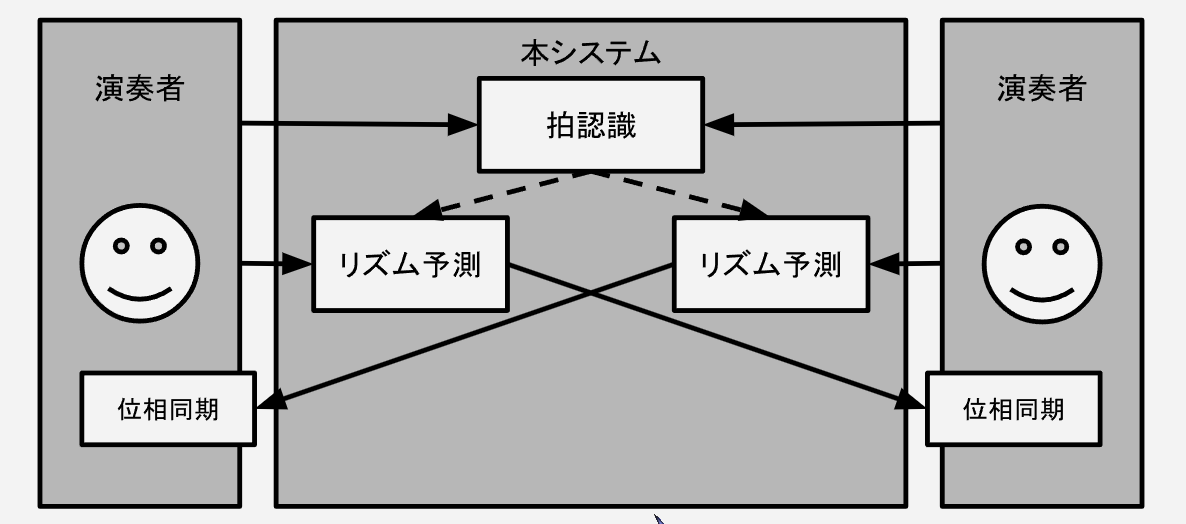
\includegraphics[width=0.8\linewidth]{src/architecture.png}
  \caption{本システムのアーキテクチャ}
  \label{fig:architecture}
\end{figure}

\section{仮説}
遅延のあるネットワーク下でも,演奏相手の演奏を予測しながら演奏を行うことができれば,遅延の量に関係なくまるで同じ部屋にいるかのように演奏できると仮説を立てる.

従来のAdaptive Metronomeと違い,メトロノームの音ではなく予測の音を再生することで演奏者はまるで人間の演奏相手と演奏しているかと同等の体験を得られることができると考える.
本システムを用いると音楽における音のニュアンス,表現を保ちつつ,遅延の補償を行うことができる.
なお音楽的な表現を保つことが目的であるため,表現を伝達するのに十分な予測精度を得られればよいと考える.

%%% Local Variables:
%%% mode: japanese-latex
%%% TeX-master: "../bthesis"
%%% End:
